\section{Model description} \label{Model-description}
\subsection{Reactor design}

The Single-fluid Double-zone Thorium-based Molten Salt Reactor (SD-TMSR) design was proposed by the Chinese Academy of Sciences in 2011 
\cite{li_optimization_2018,jiang2012advanced,li2015analysis,li2017model}. The \gls{SD-TMSR} is a graphite-moderated molten salt reactor with a thermal power of 2250 MW$_{th}$. The 
design of the \gls{SD-TMSR} is inspired by the \gls{MSBR} 
\cite{robertson_conceptual_1971} and the \gls{TMSR} \cite{nuttin2005potential} after modifying the geometry to 
control the positive temperature coefficient in the MSBR. The \gls{SD-TMSR} core 
geometry is described in detail by Li \emph{et al.} and Ashraf \emph{et al.}
\cite{li_optimization_2018,ashraf2019whole_core}. The active zone of the \gls{SD-TMSR} is a right cylinder divided into the inner zone (486 fuel tubes) and the outer zone (522 fuel tubes) to enhance breeding performance.

In this study, the fuel salt composition is 70LiF - 17.5BeF$_2$ - 12.5(HM)F$_4$ mole\%, where HM is the heavy metal (i.e. $^{232}$Th and fissile materials). Three different types of initial fissile materials are considered: (1) $^{233}$U \cite{ashraf2019whole_core}, (2) reactor-grade Pu \cite{marka1993explosive}, and (3) transuranic (TRU) elements from \gls{LWR} LWR \gls{SNF} \cite{de2000scenarios}.
The density and volume of the fuel salt are 3.3 g/cm$^{3}$ and 52.9 m$^3$, respectively.
The liquid fuel salt circulates continuously through the fuel tubes that pierce the graphite hexagonal 
prisms. The active zone is surrounded by axial and radial graphite reflectors to minimize the neutron leakage. Finally, the \gls{SD-TMSR} pressure vessel holds all reactor components and is made of a Hastelloy N alloy. The main 
characteristics of the \gls{SD-TMSR} are summarized in Table~\ref{tab:table1}.


\begin{table}  %[!ht]
	\caption{The main characteristics of the SD-TMSR \cite{li_optimization_2018}.}
	\vspace{0.1in}
	\begin{tabularx}{\textwidth}{l | l}
		\hline
		Thermal power, MW$_{th}$          				&  2,250  \\ 
		Fuel salt components                            & LiF-BeF$_2$-(\gls{HM})F$_4$ \\
		Fuel composition, mole\%                        & 70-17.5-12.5    \\
		$^7$Li enrichment, \%        				& 99.995   \\
		Fuel temperature, K 							& 900  \\
		Fuel density at 900 K, g/cm$^3$		  		& 3.3 \\
		Fuel dilatation coefficient, g/(cm$^3$$.$K)  &  -6.7$\times$10$^{-4}$ \\
		Graphite density, g/cm$^3$             	    & 2.3	\\  
		B$_4$C density, g/cm$^3$					& 2.52  \\
		$^{10}$B enrichment, \%						&  18.4  \\
		Core diameter, cm								& 460  \\
		Core height, cm									& 460  \\
		Side length of the graphite hexagonal prism, cm   & 7.5 \\
		Inner radius, cm							& 3.5  \\
		Outer radius, cm							& 5  \\
		Ratio of molten salt and graphite in the inner zone	&  0.357  \\
		Ratio of molten salt and graphite in the outer zone &  1.162  \\
		Fuel volume, m$^3$  &	52.9 \\
		\hline
	\end{tabularx}
	\label{tab:table1}
\end{table}
%%%%%%%%%%%%%%%%%%%%%%%%%%%%%%%%%%%%%%%%


\subsection{Control rod design} \label{CRD}

The reactivity of the SD-TMSR core is controlled through two systems of control assemblies:
\begin{enumerate}
\item The Control Safety Devices (CSD), and
\item The Shutdown Safety Devices (SSD).
\end{enumerate}
The CSD system is designed for reactivity control during normal operation and the SSD system is designed for an emergency reactor shutdown.
In the present work, five different absorber materials are considered based on their neutronics and safety performance:
\begin{enumerate}
\item B$_4$C with boron enriched to 90\% $^{10}$B isotope,
\item hafnium diboride (HfB$_2$),
\item hafnium hydride (HfH$_{1.62}$),
\item gadolinium oxide (Gd$_2$O$_3$), and
\item europium oxide (Eu$_2$O$_3$).
\end{enumerate}
Boron carbide (B$_4$C) is widely used in control rods fabrication. Enriching B$_4$C increases the fraction of highly neutron absorber isotope (i.e. $^{10}$B) and helps to reach the necessary absorptivity. However, issues related to helium gas release through (n,$\alpha$) reactions of $^{10}$B, swelling, melting risk, and high loss of the reactivity worth limit the B$_4$C lifespan \cite{guo2019optimized}. Hafnium and rare earth elements oxides absorb neutrons through (n,$\gamma$) reactions and this limits gas emission.

The control rod is a cylinder with a radius of 0.75 cm and a height of 520 cm. The absorber material is surrounded by a 0.25-cm-thick clad made of AIM1 (15Cr-15Ni) steel alloy \cite{SERAN2017285} and the rod follower is made of SiC structural material (see Figure~\ref{fig:cr}). A small gap between the cladding and rod follower is considered to facilitate the control rod movement.

Since the total quantity and distribution of the SD-TMSR control assemblies are unknown, we proposed an original distribution as a starting point of this analysis. We added clusters consist of four control rods to specific graphite hexagonal prisms (elements) in the SD-TMSR core. Every four control rods (cluster) can move together as one group. Figure~\ref{fig:graphite_elemen} and~\ref{fig:graphite_elemen1} demonstrate the plan and axial view of the graphite element with the four control rods. The total numbers of graphite elements with control rods are 25: 16 CSD and 9 SSD.

\begin{figure}[t!]  % replace 't' with 'b' to \centering
	\centering
	\hspace{+0.65in} 
	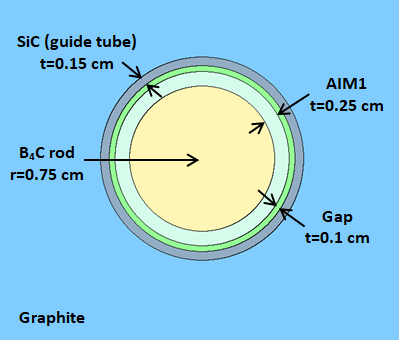
\includegraphics[width=\textwidth]{cr.png}
	\caption{Cross section of the B$_4$C control rod.}
	\label{fig:cr}
\end{figure}

\begin{figure}[t!]  % replace 't' with 'b' to \centering
	\centering
	\hspace{+0.65in}
	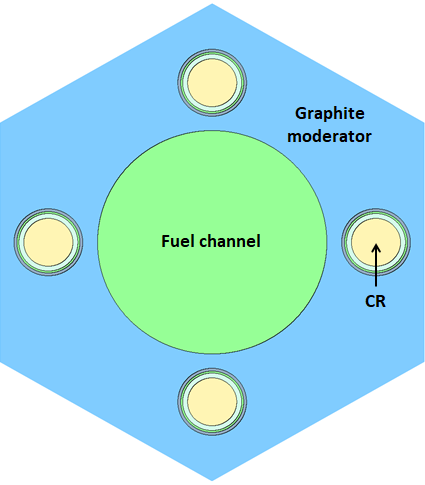
\includegraphics[width=\textwidth]{graphite_element.png}
	\caption{Graphite element with the four control rods (cluster) located at the same distance from the fuel channel.}
	\label{fig:graphite_elemen}
\end{figure}

\begin{figure}[t!]  % replace 't' with 'b' to \centering
	\centering
	\hspace{+0.65in}
	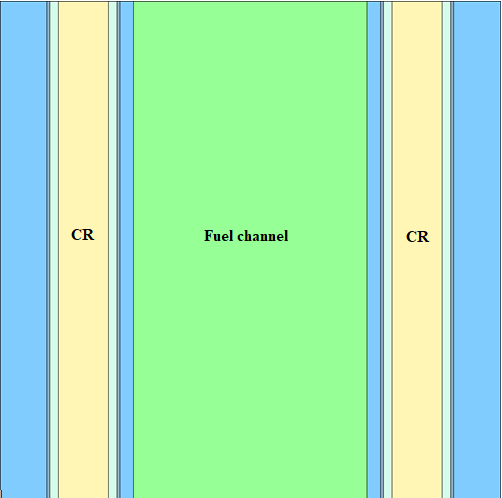
\includegraphics[width=\textwidth]{graphite_element1.png}
	\caption{Axial view of graphite element with control rods.}
	\label{fig:graphite_elemen1}
\end{figure}

Figure~\ref{fig:core_25} illustrates the numbering scheme of control rods clusters in the SD-TMSR core.
The CSD1-16 clusters are represented as yellow color and distributed as two rings: inner and outer ring (peripheral ring). The inner ring includes CSD from 1 to 6, while the outer ring includes CSD from 7 to 16. Red color stands for SSD1-9 clusters.
We distributed the graphite elements with control rods clusters homogeneously in the inner core of the SD-TMSR, where the moderator-to-fuel ratio is high.
The selected core segment in the above corner of the Figure~\ref{fig:core_25} shows that both CSD and SSD clusters consist of four control rods located at the same distance from the fuel channel.

\begin{figure}[t!]  % replace 't' with 'b' to \centering
	\centering
	\hspace{+0.65in}
	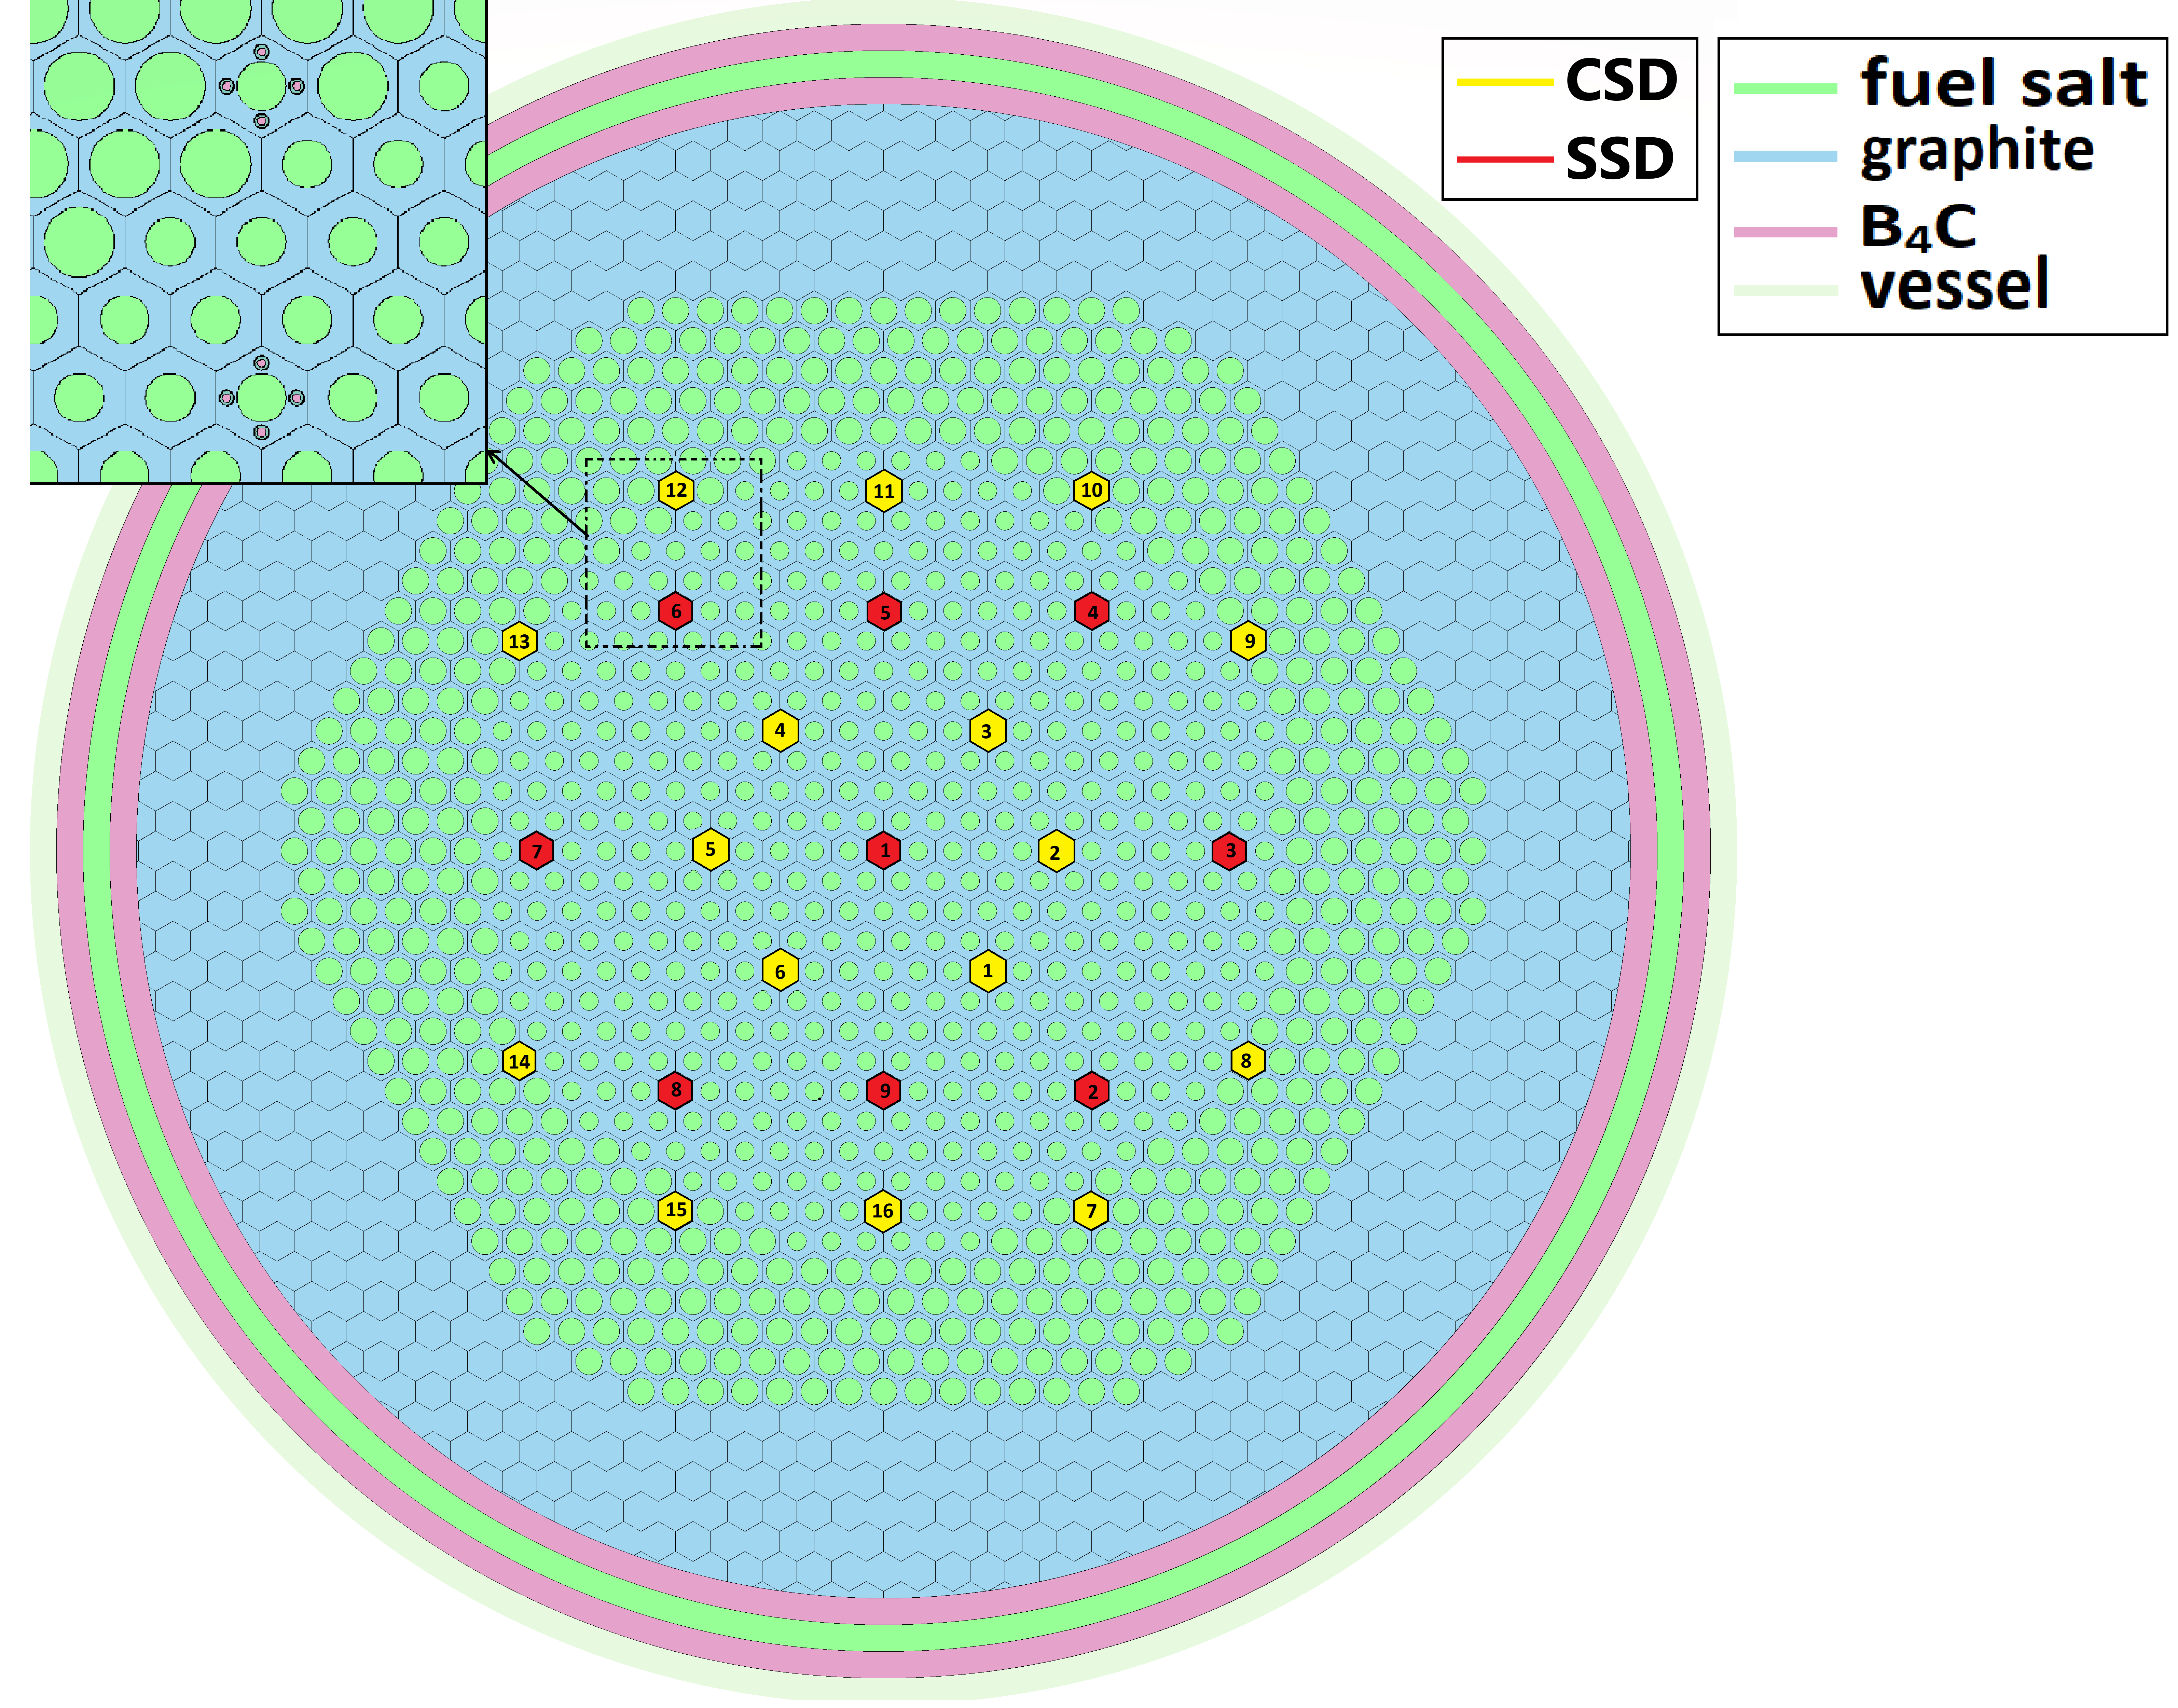
\includegraphics[width=\textwidth]{core_25.png}
	\caption{Distribution of the graphite elements with control rods in the SD-TMSR core.}
	\label{fig:core_25}
\end{figure}


\section{Methodology and tools} \label{Methodology-and-tools}
\subsection{Control rod design evaluation}

In this work, SERPENT-2 version 2.1.31 \cite{leppanen2014serpent} is used to perform steady state calculations for the full-core of the Single-fluid Double-zone Thorium-based Molten Salt Reactor (SD-TMSR) with control rod design. We adopted the ENDF-VII.0 cross section library for all calculations in the present work. The results demonstrate whole-core runs of $12.5\times 10^6$ neutron histories per depletion step. The statistical error in $k_{eff}$ from SERPENT-2 output is equal to $\pm$ $25$ $pcm$.

The initial calculation state of the SD-TMSR is identified by normal operation conditions (see Table~\ref{tab:table1}) and fully withdrawn control rods clusters. In this case, the control rods are located above the upper plenum as shown in Figure~\ref{fig:core_26}. To validate the proposed control rods system we adopted the same operation conditions (as in the initial case) and changed the position of the control rod clusters along $Z$ direction. The main calculated parameters including reactivity, control rod worth, and interference effects (shadowing effects) will describe in the following parts.

\begin{figure}[t!] % replace 't' with 'b' to \centering
	\centering
	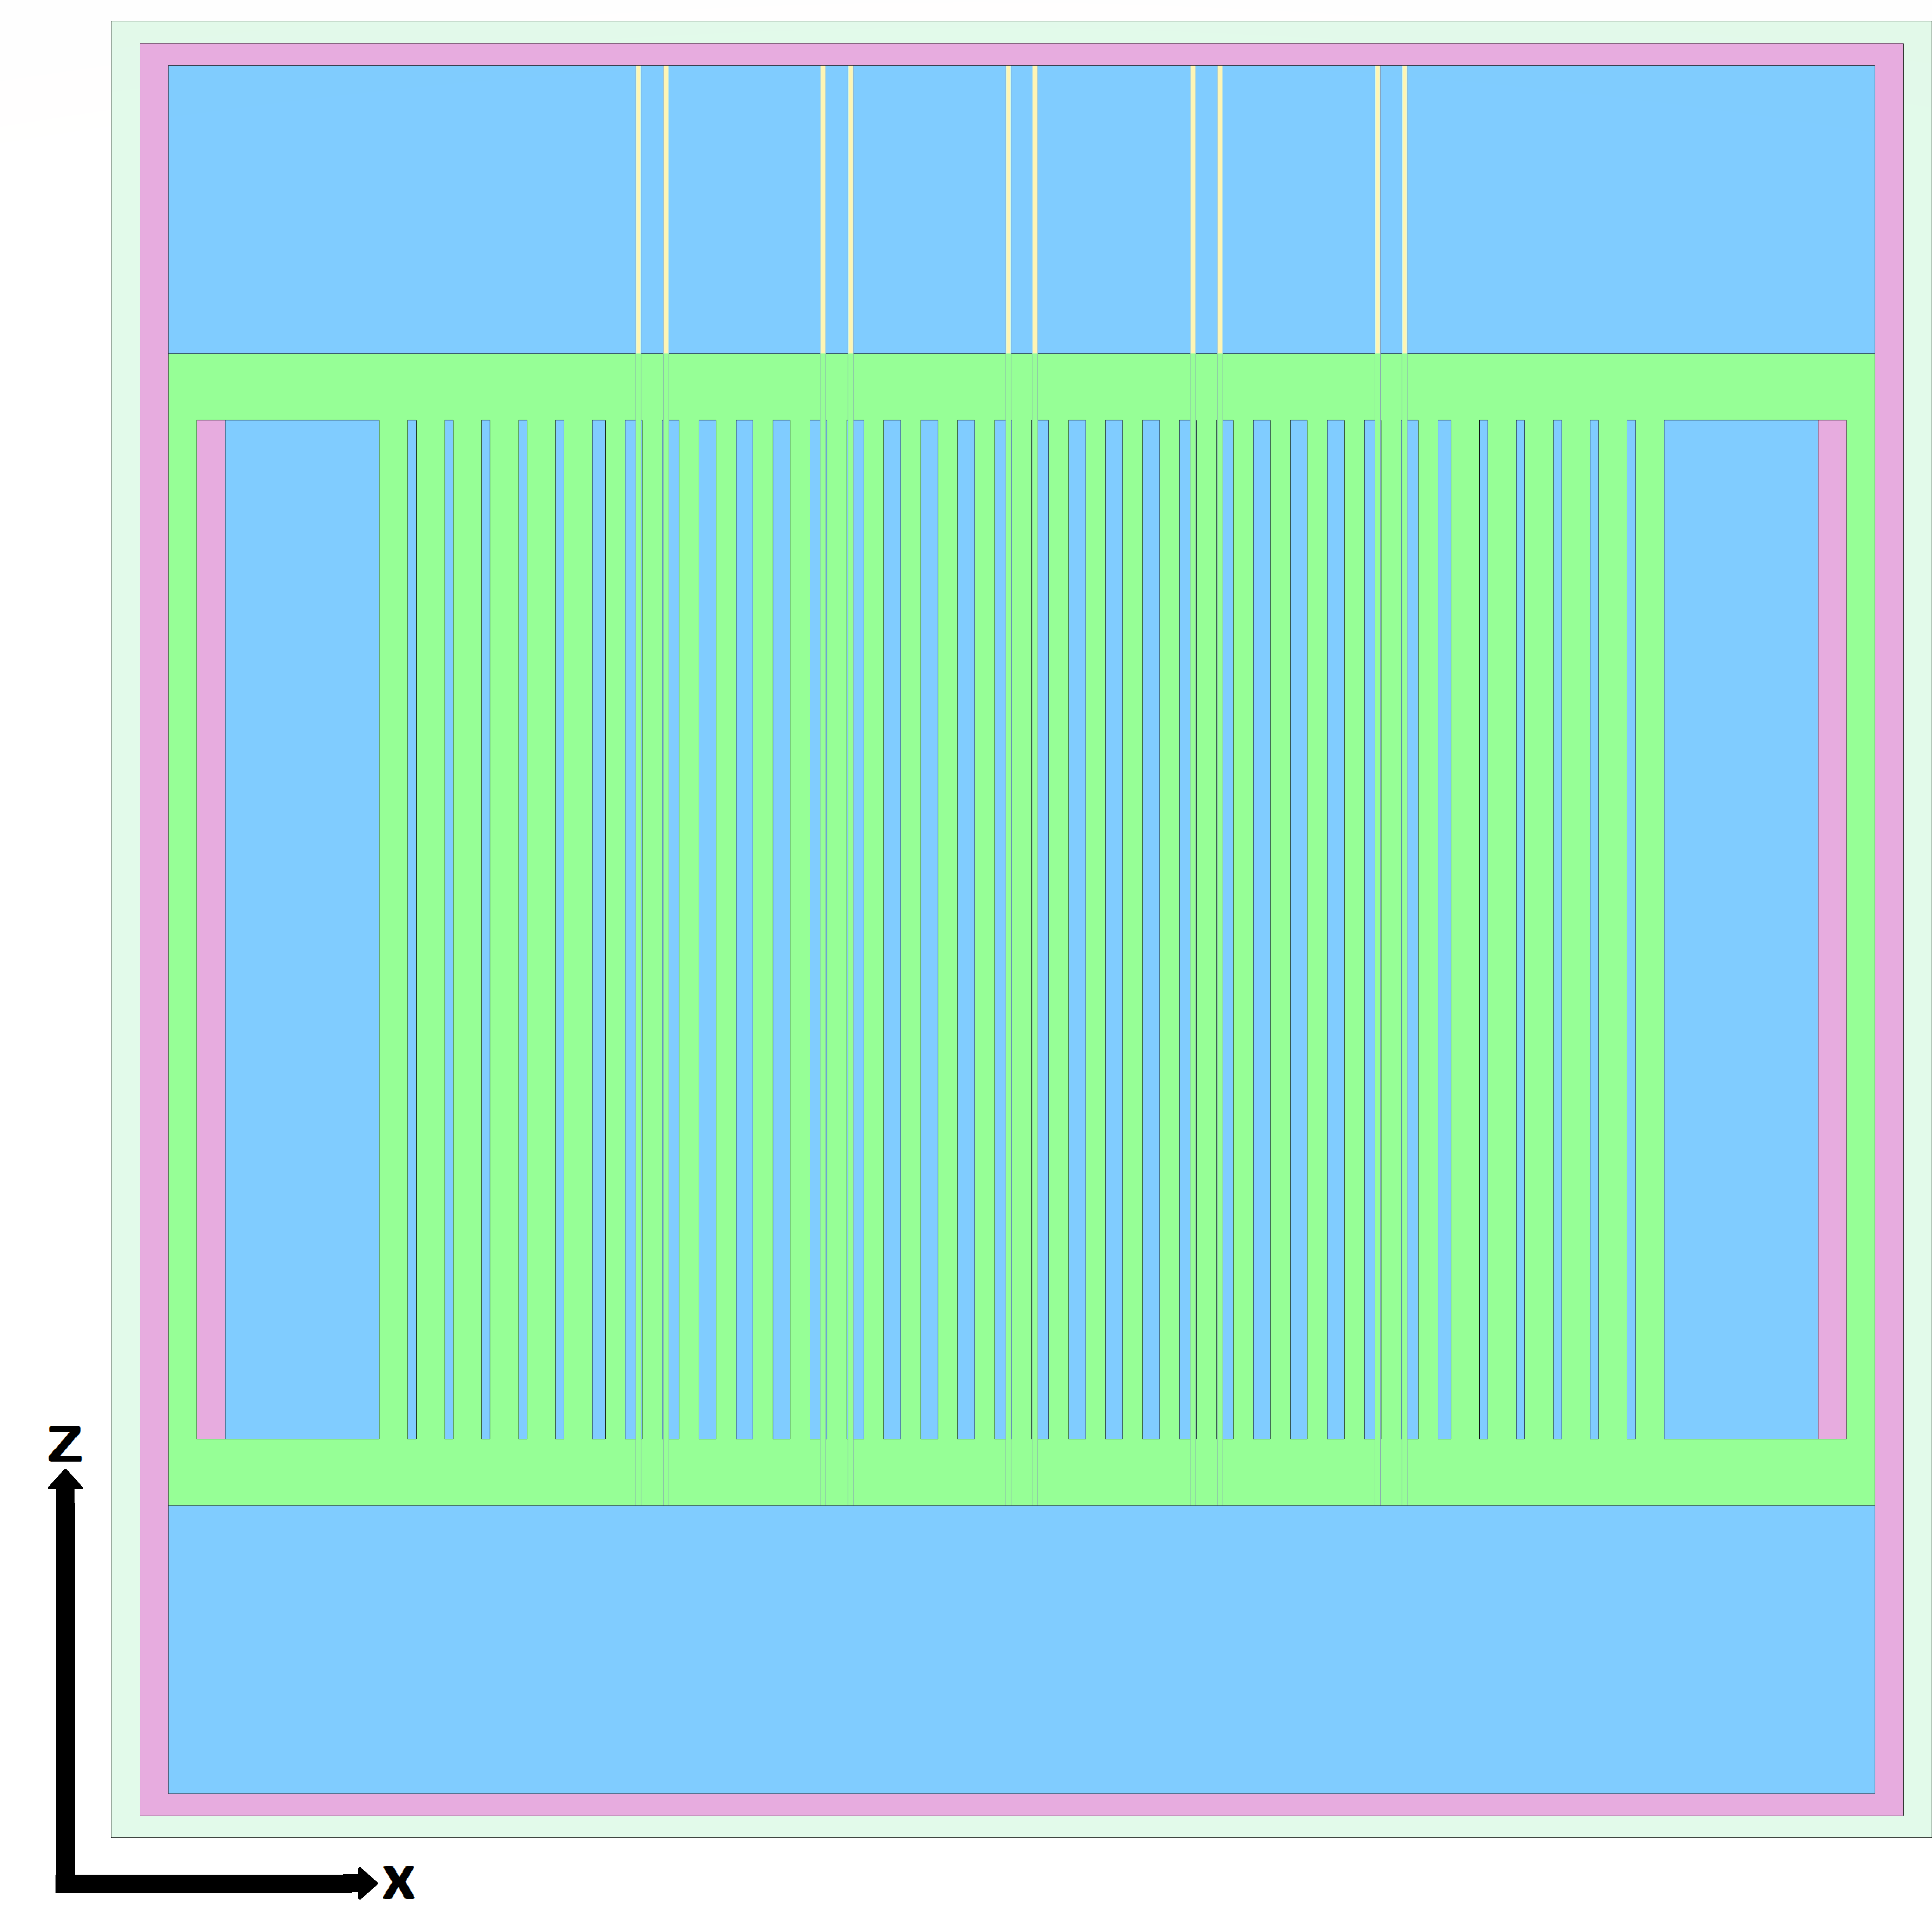
\includegraphics[width=\textwidth]{core_26.png}
	\caption{$XZ$ section of the full-core model of the SD-TMSR, CRs are fully withdrawn.}
	\label{fig:core_26}
\end{figure}

\subsubsection{Reactivity calculation}

The excess reactivity $\rho$$_e$ is the reactivity of the core when all control rods are withdrawn. $\rho$$_e$ is calculated by SERPENT-2 in \$ units based on equation~\ref{Equ:1}, where $k_{eff}$ is the effective multiplication factor of the core and $\beta_{eff}$ is the effective fraction of delayed neutrons. The effective delayed neutron fraction is calculated by the adjoint-weighted time constants using perturbation technique in SERPENT-2 \cite{leppanen2014calculation}.

\begin{equation}
\label{Equ:1}
{{\rho}_{e}}=\dfrac{{k_{eff}}-1}{{k_{eff}}{{\beta}_{eff}}},
\end{equation}

\subsubsection{The control rod worths (CRW)}

The control rod worth (CRW) is the amount of negative reactivity that associated with the control rod insertion. The CRW is calculated by SERPENT-2 in \$ units based on equation~\ref{Equ:2}, where $\Delta\rho$$_{CRi}$ is the worth of i$^{th}$ CR, $\rho$$_e$ is the initial excess reactivity, and $\rho$$_{CRi}$ is the excess reactivity after i$^{th}$ CR insertion \cite{vcerba2017optimization}.

\begin{equation}
\label{Equ:2}
{{\Delta}{\rho}_{CRi}}={{\rho}_{e}}-{{\rho}_{CRi}},
\end{equation}

\subsubsection{Shutdown Margin (SDM)}

The shutdown margin (SDM) is the amount of reactivity by which a full reactor core is subcritical from a given state. The SDM is expressed in terms of reactivity and calculated by equation~\ref{Equ:6}, where $\Delta\rho_{SSD}$ is the total worth of the Shutdown Safety Devices (SSD) and $\rho$$_e$ is the core excess reactivity.

\begin{equation}
\label{Equ:6}
{SDM}={{\Delta}{\rho}_{SSD}}-{{\rho}_{e}},
\end{equation}

\subsubsection{Interference effects (shadowing effects)}

Interference between control rods (CRs) or shadowing effects occurs when one (or more) control rod affects the reactivity worth of another control rod in the surroundings. Thus, anti-shadowing is observed when the combined rod worth is greater than the sum of the individual worths, however, the shadowing effect appears when the combined rod worth is less than the sum of the individual worths.
The core height-to-diameter ratio (H/D) and the three-dimensional configuration of the control rods affect the degree of the interference between CRs \cite{girardin2007control}. 

The amplification factor (A$_{CRi}$) of i$^{th}$ control rod helps to evaluate the shadowing effects between control rod clusters. The amplification factor is calculated by equation~\ref{Equ:3} \cite{girardin2007control,vcerba2017optimization}, where $\Delta\rho$$_{CR(1,2,\ldots N)}$ is the total worth of all control rods (from $1$ to $N$), $\Delta\rho$$_{CR(1,2,\ldots N-i)}$ is the total worth of all CRs except the investigated one i$^{th}$ and $\Delta\rho$$_{CRi}$ the worth of the i$^{th}$ rod.

\begin{equation}
\label{Equ:3}
{{A}_{CRi}}=\dfrac{{{\Delta}{\rho}_{CR(1,2,\ldots N)}}-{{\Delta}{\rho}_{CR(1,2,\ldots N-i)}}}{{\Delta}{\rho}_{CRi}},
\end{equation}

If A$_{CRi}$ is $<$1, the control rod worth is reduced due to shadowing effects, while if A$_{CRi}$ is $>$1 the control rod worth is amplified and anti-shadowing effects occur. A$_{CRi}$ = 1 means no shadowing effects occur.

\subsubsection{Integral and differential control rod worth}

The integral CRW is the total reactivity change due to control rod insertion or withdrawal. However, the differential CRW is the amount of reactivity inserted per unit of withdrawal [$\$/cm$]. We change the position of CRs clusters parallel to the z-axis from top to the bottom of the core. Equation~\ref{Equ:4} is used to calculate the integral CRW [\$], where $k_{i}$ and $k_{i-1}$ are the effective multiplication factor after and before CR insertion to i$^{th}$ step. $\beta_{i}$ is the effective fraction of delayed neutrons at i$^{th}$ step. N is the number of steps.

\begin{equation}
\label{Equ:4}
{{\Delta}{\rho}_{i}}=\sum_{i=1}^{N}\dfrac{{k_{i}}-{k_{i-1}}}{{{k_{i}}{k_{i-1}}}{{\beta}_{i}}},
\end{equation}

Equation~\ref{Equ:5} is used to calculate the differential CRW [\$/cm], where $\Delta H$ is the height change of control rod [cm] before and after insertions.

\begin{equation}
\label{Equ:5}
\dfrac{{\partial}{\rho}_{i}}{{\partial{H}}}=\dfrac{1}{{\Delta}{H}}\dfrac{{k_{i}}-{k_{i-1}}}{{{k_{i}}{k_{i-1}}}{{\beta}_{i}}},
\end{equation}


